\documentclass[journal,12pt,twocolumn]{IEEEtran}

\usepackage{setspace}
\usepackage{gensymb}

\singlespacing


\usepackage[cmex10]{amsmath}

\usepackage{amsthm}

\usepackage{mathrsfs}
\usepackage{txfonts}
\usepackage{stfloats}
\usepackage{bm}
\usepackage{cite}
\usepackage{cases}
\usepackage{subfig}

\usepackage{longtable}
\usepackage{multirow}
\DeclareMathOperator{\taninv}{tan\,inverse}
\usepackage{enumitem}
\usepackage{mathtools}
\usepackage{steinmetz}
\usepackage{tikz}
\usepackage{circuitikz}
\usepackage{verbatim}
\usepackage{tfrupee}
\usepackage[breaklinks=true]{hyperref}
\usepackage{graphicx}
\usepackage{tkz-euclide}
\usepackage{float}

\usetikzlibrary{calc,math}
\usepackage{listings}
    \usepackage{color}                                            %%
    \usepackage{array}                                            %%
    \usepackage{longtable}                                        %%
    \usepackage{calc}                                             %%
    \usepackage{multirow}                                         %%
    \usepackage{hhline}                                           %%
    \usepackage{ifthen}                                           %%
    \usepackage{lscape}     
\usepackage{multicol}
\usepackage{chngcntr}

\DeclareMathOperator*{\Res}{Res}

\renewcommand\thesection{\arabic{section}}
\renewcommand\thesubsection{\thesection.\arabic{subsection}}
\renewcommand\thesubsubsection{\thesubsection.\arabic{subsubsection}}

\renewcommand\thesectiondis{\arabic{section}}
\renewcommand\thesubsectiondis{\thesectiondis.\arabic{subsection}}
\renewcommand\thesubsubsectiondis{\thesubsectiondis.\arabic{subsubsection}}


\hyphenation{op-tical net-works semi-conduc-tor}
\def\inputGnumericTable{}                                 %%

\lstset{
%language=C,
frame=single, 
breaklines=true,
columns=fullflexible
}
\begin{document}
\newtheorem{theorem}{Theorem}[section]
\newtheorem{problem}{Problem}
\newtheorem{proposition}{Proposition}[section]
\newtheorem{lemma}{Lemma}[section]
\newtheorem{corollary}[theorem]{Corollary}
\newtheorem{example}{Example}[section]
\newtheorem{definition}[problem]{Definition}

\newcommand{\BEQA}{\begin{eqnarray}}
\newcommand{\EEQA}{\end{eqnarray}}
\newcommand{\define}{\stackrel{\triangle}{=}}
\bibliographystyle{IEEEtran}
\providecommand{\mbf}{\mathbf}
\providecommand{\pr}[1]{\ensuremath{\Pr\left(#1\right)}}
\providecommand{\qfunc}[1]{\ensuremath{Q\left(#1\right)}}
\providecommand{\sbrak}[1]{\ensuremath{{}\left[#1\right]}}
\providecommand{\lsbrak}[1]{\ensuremath{{}\left[#1\right.}}
\providecommand{\rsbrak}[1]{\ensuremath{{}\left.#1\right]}}
\providecommand{\brak}[1]{\ensuremath{\left(#1\right)}}
\providecommand{\lbrak}[1]{\ensuremath{\left(#1\right.}}
\providecommand{\rbrak}[1]{\ensuremath{\left.#1\right)}}
\providecommand{\cbrak}[1]{\ensuremath{\left\{#1\right\}}}
\providecommand{\lcbrak}[1]{\ensuremath{\left\{#1\right.}}
\providecommand{\rcbrak}[1]{\ensuremath{\left.#1\right\}}}
\theoremstyle{remark}
\newtheorem{rem}{Remark}
\newcommand{\sgn}{\mathop{\mathrm{sgn}}}
\providecommand{\abs}[1]{\vert#1\vert}
\providecommand{\res}[1]{\Res\displaylimits_{#1}} 
\providecommand{\norm}[1]{\lVert#1\rVert}
%\providecommand{\norm}[1]{\lVert#1\rVert}
\providecommand{\mtx}[1]{\mathbf{#1}}
\providecommand{\mean}[1]{E[ #1 ]}
\providecommand{\fourier}{\overset{\mathcal{F}}{ \rightleftharpoons}}
%\providecommand{\hilbert}{\overset{\mathcal{H}}{ \rightleftharpoons}}
\providecommand{\system}{\overset{\mathcal{H}}{ \longleftrightarrow}}
	%\newcommand{\solution}[2]{\textbf{Solution:}{#1}}
\newcommand{\solution}{\noindent \textbf{Solution: }}
\newcommand{\cosec}{\,\text{cosec}\,}
\providecommand{\dec}[2]{\ensuremath{\overset{#1}{\underset{#2}{\gtrless}}}}
\newcommand{\myvec}[1]{\ensuremath{\begin{pmatrix}#1\end{pmatrix}}}
\newcommand{\mydet}[1]{\ensuremath{\begin{vmatrix}#1\end{vmatrix}}}
\numberwithin{equation}{subsection}
\makeatletter
\@addtoreset{figure}{problem}
\makeatother
\let\StandardTheFigure\thefigure
\let\vec\mathbf
\renewcommand{\thefigure}{\theproblem}
\def\putbox#1#2#3{\makebox[0in][l]{\makebox[#1][l]{}\raisebox{\baselineskip}[0in][0in]{\raisebox{#2}[0in][0in]{#3}}}}
     \def\rightbox#1{\makebox[0in][r]{#1}}
     \def\centbox#1{\makebox[0in]{#1}}
     \def\topbox#1{\raisebox{-\baselineskip}[0in][0in]{#1}}
     \def\midbox#1{\raisebox{-0.5\baselineskip}[0in][0in]{#1}}
\vspace{3cm}
\title{ASSIGNMENT 3}
\author{RONGALA ARUN SIDDARDHA \\ AI20BTECH110019}
\maketitle
\newpage
\bigskip
\renewcommand{\thefigure}{\theenumi}
\renewcommand{\thetable}{\theenumi}
Download all python codes from 
\begin{lstlisting}
https://github.com/ArunSiddardha/EE3900/blob/main/Assignment_2/code/Assignment_3.py
\end{lstlisting}
%
and latex-tikz codes from 
%
\begin{lstlisting}
https://github.com/ArunSiddardha/EE3900/blob/main/Assignment_2/Assignment_3.tex
\end{lstlisting}
%
\section{Ramsey/tangent and normals/ Q.19}
Prove that the circle $\vec{x}^\top\vec{x}-\myvec{6 & 4}\vec{x} + 9$ subtends an angle $\tan^{-1}{\frac{12}{5}}$ at the origin
%
\section{Solution}
The general equation of a second dergree can be expressed as :
\begin{align}
    \vec{x}^\top\vec{V}\vec{x}+2\vec{u}^\top\vec{x} + f = 0 
\end{align}

We know that, for a circle,
\begin{align}
    \vec{V} = \vec{I}\\
    \vec{c} = -\vec{u}
\end{align}
\begin{align}
   \vec{u} = \myvec{-3 \\ -2}, f=9\\
   \vec{c}=\myvec{3 \\ 2}\\
    \vec{u}=\myvec{-3 &-2}^\top 
\end{align}
The points of contact $\vec{q}$, of a line with a normal vector $\vec{n}$ to the conics are given by:
\begin{align}
\vec{q} = \vec{V}^{-1}\brak{\kappa \vec{n}-\vec{u}} \label{eq:9} \\
\kappa = \pm \sqrt{\frac{\vec{u}^T\vec{V}^{-1}\vec{u}-f}{\vec{n}^T\vec{V}^{-1}\vec{n}}}\label{eq:10}
\end{align}
We know that, for a circle, 
\begin{align}
\vec{V} = \vec{I}\label{eq:11}  
\end{align}
If $r$ is radius and $\vec{c}$ is the centre of the circle we have:
\begin{align}
f &=\vec{u}^T\vec{u}-r^2  \label{eq:5} \\  
\vec{c} &=-\vec{u}
\end{align}
and from the properties of an Identity matrix, 
\begin{align}
\vec{I}^{-1} &= \vec{I} \\
\vec{I}\vec{X} &= \vec{X}   
\end{align}
\begin{align}
\kappa &= \pm \sqrt{\frac{r^2}{\vec{n}^{\top}\vec{n}}} \\
&= \pm \sqrt{\frac{4}{\vec{n}^{\top}\vec{n}}} \\
& =  \pm \frac{2}{\sqrt{\vec{n}^{\top}\vec{n}}}
\end{align}
So,
\begin{align}
    \vec{q}= \pm \frac{2 \vec{n}}{\sqrt{\vec{n}^{\top}\vec{n}}}+ \vec{u}\\
\end{align}
Now $\vec{q}$ lies on the line therefore,
\begin{align}
   \vec{n}^{\top} \brak{\pm \frac{2 \vec{n}}{\sqrt{\vec{n}^{\top}\vec{n}}}+ \vec{u} } = 0\\
   \pm 2 \sqrt{\vec{n}^{\top}\vec{n}}+ \vec{n}^{\top}\vec{u}=0
\end{align}
    Since , $ \vec{n} = \myvec{m & -1}^\top \label{eq}$ for the tangent
\begin{align}
   \implies \pm \brak{2\sqrt{m^2+1}}&=2-3m
\end{align}
\textbf{S.O.B.S}
\begin{align}
    4\brak{m^2+1}=4 + 9m^2 -12m\\
    5m^2-12m=0\\
    m(5m-12)=0\\
    m=0 \;or\; m = \frac{12}{5}
\end{align}
    \begin{figure}
        \centering
        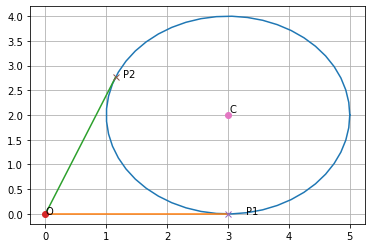
\includegraphics[width = \columnwidth]{Assignment_3.png}
        \caption{graph}
        \label{fig:my_label}
\end{figure}
So,
\begin{align}
\vec{n_1}&= \myvec{\frac{12}{5} & 1}^{\top} \;\; \vec{n_2}=\myvec{0 & 1}^{\top}\\
   \cos \theta &= \frac{\vec{n_1}^{\top}\vec{n_2}}{\norm{\vec{n_1}}\norm{\vec{n_2}}}\\
   &= \frac{\myvec{\frac{12}{5} & 1}\myvec{0 \\ 1}}{\frac{13}{5}\times 1}\\
   \cos \theta &= \frac{5}{13}
\end{align}
Therefore angle between the lines is $\tan^{-1}\brak{\frac{12}{5}}$ \\
\textbf{Hence proved.}
\end{document}